\chapter{\textsc{Results and Evaluation}}
\label{chapterlabel5}

The previous section described the methods and tools used throughout a number of development, analysis and evaluation stages including data collection, network creation and comparative analysis. It documents the journey of collecting the data and interpreting it in a way that allowed the creation of a number of networks.

This study is distinctive to other network science projects, which will make use of data that already carries a suitable network format, which enables its analysis straight away. However, in this case, as the problem is address in a novel way, the data is not already pre-processed and in a suitable format for network analysis. Therefore, part of the project and its objective concentrates on data collection and manipulation in order to be able to formulate a number of networks which can then be analysed. Furthermore, this makes the networks constructed from the collected EPSRC data very much part of the results of this project.

This section presents the results produced by the project while also covering their evaluation. The results include the networks constructed from the collected data as well as the clusters of topics and researchers identified. The current clusters are discussed and compared with historical ones which were also identified in order to discover transitional trends related to research and funding. Furthermore, different network interpretations of the data are also analysed and contrasted in order to identify which one yields a more rational clustering.

\section{Networks of Topics}

One of the sections of the Methodology chapter described the methods used in the process of creating a number of different networks from the collected data. This section presents the results of following those methods.

One of the types of network created is a Network of Topics. It consists of nodes which represent topics and edges which are interpreted in two different ways, as they can either represent grants or researchers. A separate network was constructed to fit each interpretation. They are referred to as \textit{Grants as edges} and \textit{Researchers as edges}. Moreover, as historical grant data was also collected, a further two versions of the \textit{Topic network (Grants as edges)} were constructed: 1990 to 2000 and 2000 to 2010, which resulted in a total of four constructed networks.

\subsection{Topic network (Grants as edges)}

The \textit{Topic network (Grants as edges)} constructed from current data consists of 223 nodes representing as many topics and 2008 edges representing common grants between topics. Fig. \ref{fig:topic_a_vis} showcases the visualisation of this network.

\begin{figure}[htpb]
    \centering
    \fbox{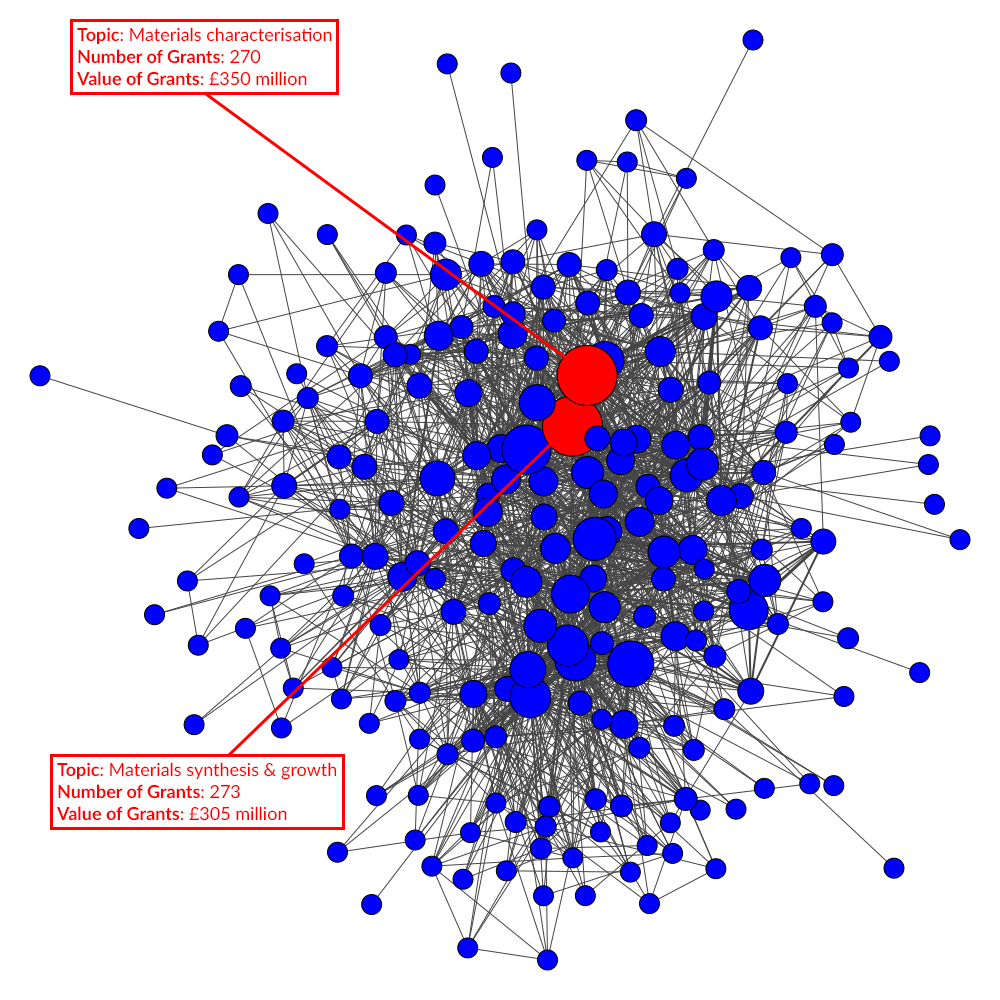
\includegraphics[width=12.5cm]{networks/topic_a}}
    \caption[Visualisation of Topic network (Grants as edges) constructed using the current data set (2010 to 2016)]{Visualisation of Topic network (Grants as edges) constructed using the current data set (2010 to 2016). Nodes coloured in red represent the topics involved in most grants.}
    \label{fig:topic_a_vis}
\end{figure}

In comparison, both historical networks have less nodes with the \textit{2000 to 2010} and \textit{1990 to 2010} networks consisting of 208 and 136 nodes, respectively. This is expected, as the number of initial disciplines was lower, and gradually increased with time. Interestingly, the \textit{2000 to 2010} network consists of more edges which transitions into more topics being connected to each through common grants. However, the increased number of edges also seems to have some correlation to the fact that the network is unconnected, while the other two are connected. This occurs when an edge does not exist between every pair of nodes. Furthermore, all networks are weighted and the edge weight represents the number of grants that two topics have in common. Table \ref{table:topic_a_stats} presents the statistics of the Topic networks (Grants as edges).

\begin{table}[!htbp]
\centering
\caption[Statistics of the Topic network (Grants as edges) constructed using both the historical (1990 to 2010) and current (2010 to 2016) data sets.]{Statistics of the Topic network (Grants as edges) constructed using both the historical (1990 to 2010) and current (2010 to 2016) data sets.}
\label{table:topic_a_stats}
\begin{tabular}{r|rrr}
{} & \textbf{1990-2000} & \textbf{2000-2010} & \textbf{2010-2016}\\
\hline\\
\textbf{Nodes}                          & {136}     & {208}     & {223}\\
\textbf{Edges}                          & {748}     & {3592}    & {2008}\\
\textbf{Type}                           & {Undirected} & {Undirected} & {Undirected}\\
\textbf{Weighted}                       & {Yes}     & {Yes}     & {Yes}\\
%\textbf{Connected}                     & {Yes}     & {No}      & {Yes}\\
\textbf{Average Degree}                 & {11}      & {34.538}  & {18.009}\\
\textbf{Average Weighted Degree}        & {12.721}  & {35.337}  & {19.543}\\
\textbf{Diameter}                       & {6}       & {5}       & {5}\\
%\textbf{Radius}                        & {3}       & {1}       & {3}\\
\textbf{Density}                        & {0.081}   & {0.167}   & {0.081}\\
\textbf{Modularity}                     & {0.4}     & {0.271}   & {0.373}\\
%\textbf{Communities}                   & {5}       & {5}       & {6}\\
\textbf{Weak Components}                & {1}       & {2}       & {1}\\
%\textbf{Node Closeness}                & {0.392}   & {0.245}   & {0.423}\\
%\textbf{Node Betweenness}              & {108.536} & {109.776} & {156.483}\\
%\textbf{Edge Betweenness}              & {32.007}  & {12.235}  & {29.706}\\
\textbf{Average Clustering Coefficient} & {0.453}   & {0.59}    & {0.597}\\
%\textbf{Eigenvector Centrality}        & {0.105}   & {0.232}   & {0.204}\\
\textbf{Average Path Length}            & {2.54}    & {2.077}   & {2.395}\\
\end{tabular}
\end{table}

\subsection{Topic network (Researchers as edges)}

The \textit{Topic network (Researchers as edges)} represents the second interpretation of the data, and is formed of topics represented by 225 nodes connected by 5192 edges. Fig. \ref{fig:topic_b_vis} showcases the visualisation of this network. The substantial increase in edges compared to the \textit{Grants as edges} interpretation, is in part due to the fact that the number of researcher records exceeds the number of grant records by 2699 records. This network is also weighted, but on this occasion, the edge weight represents the number of researchers two topics have in common.

\begin{figure}[htpb]
    \centering
    \fbox{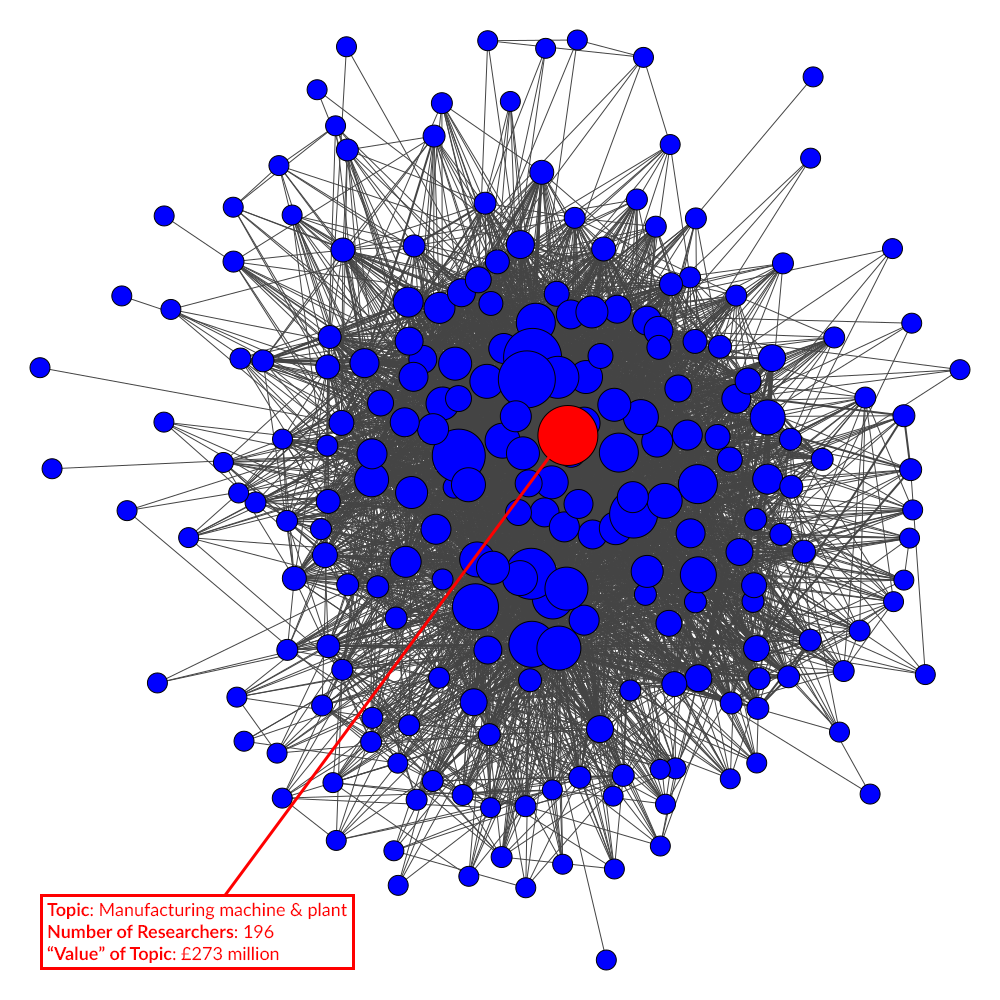
\includegraphics[width=12.5cm]{networks/topic_b}}
    \caption[Visualisation of Topic network (Researchers as edges)]{Visualisation of Topic network (Researchers as edges). Node coloured in red represents the topic contained by most researchers.}
    \label{fig:topic_b_vis}
\end{figure}

It is essential to indicate the slight difference in the number of nodes between the \textit{Grants as edges} and \textit{Researchers as edges} interpretations. The former considers grants with two or more topics while the latter considers researchers with two or more topics. In either interpretation, records may exist where a specific topic appears in a single record and is also the single topic within that record. This means that the topic will not be considered in the analysis, as links to other topics cannot be established. Table \ref{table:topic_researchers_stats} presents the statistics of the \textit{Topic network (Researchers as edges)}.

\begin{table}[!htbp]
\centering
\caption[Statistics of the Topic network (Researchers as edges).]{Statistics of the Topic network (Researchers as edges).}
\label{table:topic_researchers_stats}
\begin{tabular}{r|r}
{} & \textbf{2010-2016}\\
\hline\\
\textbf{Nodes}                          & {225}\\
\textbf{Edges}                          & {5192}\\
\textbf{Type}                           & {Undirected}\\
\textbf{Weighted}                       & {Yes}\\
%\textbf{Connected}                     & {Yes}\\
\textbf{Average Degree}                 & {46.151}\\
\textbf{Average Weighted Degree}        & {52.436}\\
\textbf{Diameter}                       & {4.0}\\
%\textbf{Radius}                        & {2}\\
\textbf{Density}                        & {0.206}\\
\textbf{Modularity}                     & {0.234}\\
%\textbf{Communities}                   & {4}\\
\textbf{Weak Components}                & {1}\\
%\textbf{Node Closeness}                & {0.522}\\
%\textbf{Node Betweenness}              & {106.686}\\
%\textbf{Edge Betweenness}              & {9.477}\\
\textbf{Average Clustering Coefficient} & {0.715}\\
%\textbf{Eigenvector Centrality}        & {0.289}\\
\textbf{Average Path Length}            & {1.925}\\
\end{tabular}
\end{table}

\section{Clusters of Topics}

The previous section presented part of the first batch of results that the project produced which is the \textit{Networks of Topics}. The optimal solution identified at the end of the comparison experiments stage was applied to the networks constructed, which resulted in a number of topic clusters. This section presents and details the results of clustering the \textit{Grants} and \textit{Researchers as edges} interpretations of the {\textit{Topic network}.

\subsection{Topic network (Grants as edges)}

The application of the Louvain community detection algorithm on the Topic network (Grants as edges) resulted in the identification of 6 different communities of topics. Fig. \ref{fig:topic_a_current_cs} showcases the visualisation of the identified community structure within this network. Table \ref{table:topic_a_current_numbers} presents the number of nodes representing topics, the number and value of grants and the predominant words within each community in the \textit{Topic network (Grants as edges)} constructed using the current data set (2010 to 2016). The complete clustering of the Topic network (Grants as edges) constructed using the current data set (2010 to 2016) is presented in Table \ref{table:topic_a_current_clusters_appendix} which is part of Appendix \ref{appendix:data}.

\begin{figure}[htpb]
    \centering
    \fbox{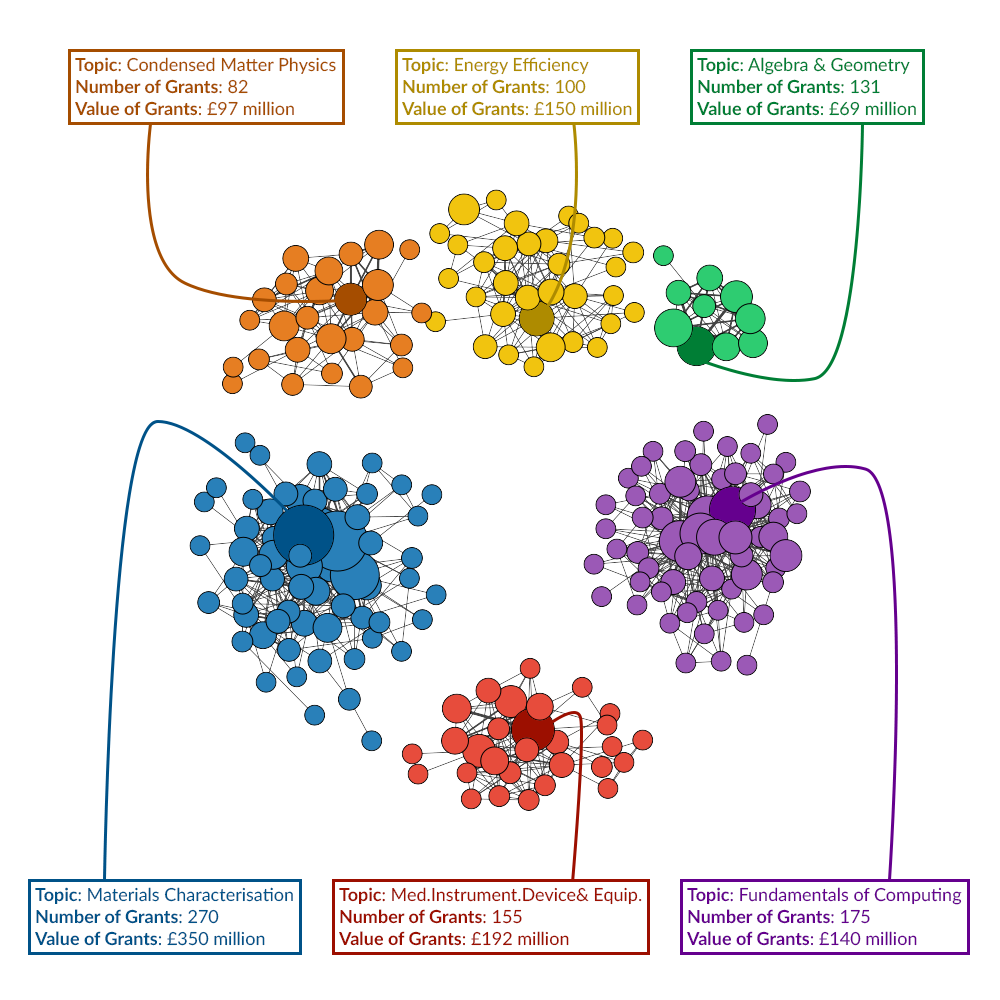
\includegraphics[width=12.5cm]{communities/topic_a_cs}}
    \caption[Visualisation of the community structure within the Topic network (Grants as edges) constructed using the current data set (2010 to 2016).]{Visualisation of the community structure within the Topic network (Grants as edges) constructed using the current data set (2010 to 2016). Node coloured darker represent the topics contained in most grants, and the topic, number of grants and value of grants are provided.}
    \label{fig:topic_a_current_cs}
\end{figure}

\begin{table}[!htbp]
\centering
\caption[Number of nodes and grants, value of grants and the predominant words of each community in the Topic network (Grants on edges) constructed using the current data set (2010 to 2016).]{Number of nodes and grants, value of grants and the predominant words based on word frequency of each community identified in the Topic network (Grants on edges) constructed using the current data set (2010 to 2016). The number of grants includes duplicate grants, as a grant can be part of more than one community. Subsequently, the value of grants also includes the duplicate grants. However, the last column represents the number and value of unique grants in communities within the current Topic network (Grants on edges).}
\label{table:topic_a_current_numbers}
\begin{tabular}{r|>{\raggedleft\arraybackslash}p{1.6cm}>{\raggedleft\arraybackslash}p{1.6cm}>{\raggedleft\arraybackslash}p{1.6cm}>{\raggedleft\arraybackslash}p{6.4cm}}
{} & \textbf{Number (topics)} & \textbf{Number (grants)} & \textbf{Value (grants)} & \textbf{Predominant words based on frequency of words}\\
\hline\\
\textbf{C1}  & {29}  & {511}  & {\pounds629M}  & {biology, biomedical, science}\\
\textbf{C2}  & {61}  & {774}  & {\pounds862M}  & {design, computing, psychology}\\
\textbf{C3}  & {63}  & {1338} & {\pounds1.5B}  & {chemistry, engineering, materials}\\
\textbf{C4}  & {10}  & {317}  & {\pounds332M}  & {mathematical, analysis}\\
\textbf{C5}  & {34}  & {480}  & {\pounds584M}  & {management, engineering, energy}\\
\textbf{C6}  & {26}  & {484}  & {\pounds766M}  & {optical, devices, quantum}\\
\hline\\
\textbf{All} & {223} & {3072} & {\pounds3.5B}  & {engineering, biology, chemistry}\\
\end{tabular}
\end{table}

\noindent\textbf{Community 1 (Biology \& Science)} has a clear focus surrounding biology, chemistry, medicine and science and does not consist of any topics that would be irrational to be clustered as part of it. Topics clustered within this community include: \textit{ageing: chemistry/biochemistry}, \textit{biomedical
sciences} and \textit{drug formulation \& delivery}. By far, the topic receiving most funding is \textit{med.instrument.device\& equip.}, valued at \pounds192 million. This value is justified as the topic also appears in 155 grants, more than any other in Community 1. Figure \ref{fig:topic_a_number_c1} presents a word cloud representation of Community 1.

\begin{figure}[!htbp]
    \centering
    
\includegraphics[width=13cm]{word-clouds/number/c1}
    \caption[Topics clustered within Community 1 in the Topic network (Grants as edges)]{Topics clustered within Community 1 in the Topic network (Grants as edges). Font size represents the number of grants that contain the topics.}
    \label{fig:topic_a_number_c1}
\end{figure}

\noindent\textbf{Community 2 (IT, Psychology \& Criminology)} is not as well defined as Community 1 as it consists of several topics which have obvious differences including \textit{product design}, \textit{artificial intelligence}, \textit{developmental psychology}, \textit{human communication in ict}, \textit{criminal law \& criminology} and \textit{comput./corpus linguistics}. This contrast is justified considering the significant size of the community. Furthermore, there are grants which represent a study involving a combination of two topics which are different in theory such as \textit{artificial intelligence} and \textit{linguistics}, for example. However, \textit{Natural language processing} is a field of both \textit{artificial intelligence} and \textit{computational linguistics}. Figure \ref{fig:topic_a_number_c2} presents a word cloud representation of Community 2.

\begin{figure}[!htbp]
    \centering
    
\includegraphics[width=13cm]{word-clouds/number/c2}
    \caption[Topics clustered within Community 2 in the Topic network (Grants as edges)]{Topics clustered within Community 2 in the Topic network (Grants as edges). Font size represents the number of grants that contain the topics.}
    \label{fig:topic_a_number_c2}
\end{figure}

\noindent\textbf{Community 3} also represents a comprehensible clustering enclosing topics such as \textit{fluid dynamics}, \textit{microsystems} and \textit{wind power}. It consists of three major topics both in terms of number of grants that contain them and the value of those grants: \textit{materials characterisation} (270 grants, worth \pounds350M), \textit{materials synthesis \& growth} (273 grants, worth \pounds305M) and \textit{manufacturing machine \& plant} (196 grants worth \pounds273M). Figure \ref{fig:topic_a_number_c3} presents a word cloud representation of Community 3.

\begin{figure}[!htbp]
    \centering
    
\includegraphics[width=13cm]{word-clouds/number/c3}
    \caption[Topics clustered within Community 3 in the Topic network (Grants as edges)]{Topics clustered within Community 3 in the Topic network (Grants as edges). Font size represents the number of grants that contain the topics.}
    \label{fig:topic_a_number_c3}
\end{figure}

\noindent\textbf{Community 4} is the smallest community in size (only 10 topics) but also the most well-defined community, as the topics clustered within it have a concrete, shared focus in Mathematics. It consists of research topics including \textit{algebra \& geometry}, \textit{mathematical physics} and \textit{continuum mechanics}. \textit{Algebra \& geometry} and \textit{statistics \& appl. probability} are the topics which were involved in most grants, 131 and 120, respectively. In terms of value, the latter is valued higher than the former, \pounds200M compared to \pounds69M. Figure \ref{fig:topic_a_number_c4} presents a word cloud representation of Community 4.

\begin{figure}[!htbp]
    \centering
    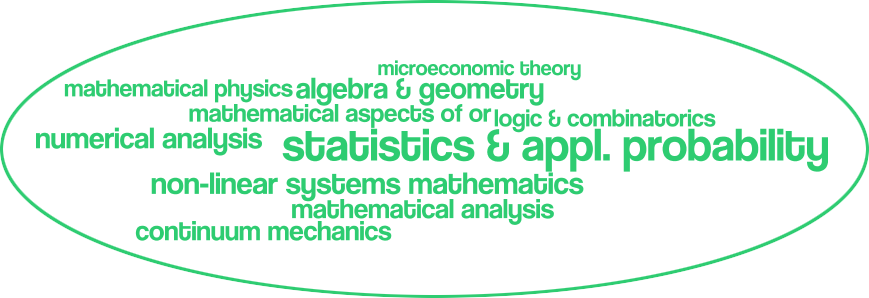
\includegraphics[width=13cm]{word-clouds/number/c4}
    \caption[Topics clustered within Community 4 in the Topic network (Grants as edges)]{Topics clustered within Community 4 in the Topic network (Grants as edges). Font size represents the number of grants that contain the topics.}
    \label{fig:topic_a_number_c4}
\end{figure}

\noindent\textbf{Community 5} represents a coherent clustering of topics including \textit{energy efficiency}, \textit{geohazards}, \textit{environment \& health} and \textit{urban \& land management}. This community represents topics from different fields which are contained in grants which share the aim to tackle an environment-related problem such as climate change or global warming. The most popular topic in terms of number of grants is \textit{energy efficiency}, with 100 grants valued at \pounds150M. Figure \ref{fig:topic_a_number_c5} presents a word cloud representation of Community 5.

\begin{figure}[!htbp]
    \centering
    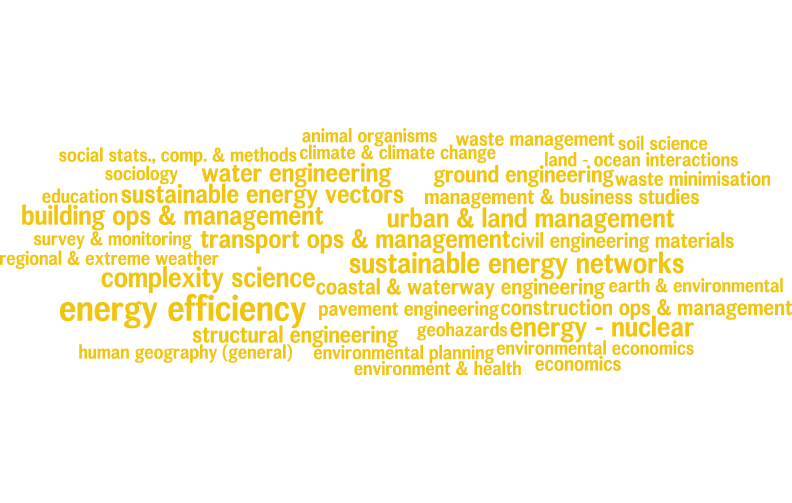
\includegraphics[width=13cm]{word-clouds/number/c5}
    \caption[Topics clustered within Community 5 in the Topic network (Grants as edges)]{Topics clustered within Community 5 in the Topic network (Grants as edges). Font size represents the number of grants that contain the topics.}
    \label{fig:topic_a_number_c5}
\end{figure}

\noindent\textbf{Community 6} is the last identified community and another community which consists of a rational clustering of topics surrounding the fields of \textit{physics} and \textit{electricity}. Topics include \textit{solar technology}, \textit{biophysics} and \textit{electronic devices \& subsys.}. \textit{Condensed Matter Physics} is involved in the highest number of grants, 82, worth \pounds97M. Figure \ref{fig:topic_a_number_c6} presents a word cloud representation of Community 6.

\begin{figure}[!htbp]
    \centering
    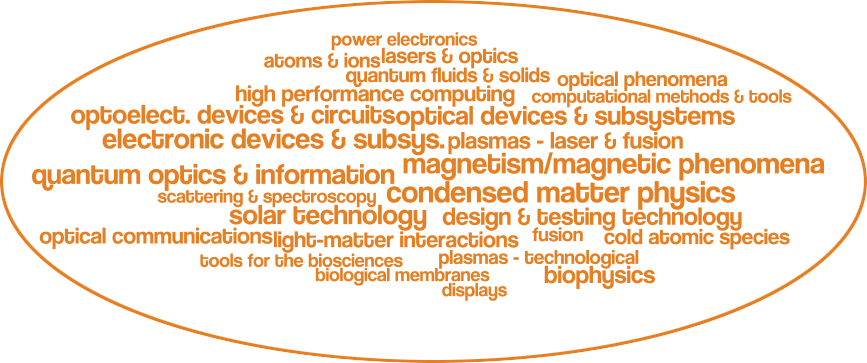
\includegraphics[width=13cm]{word-clouds/number/c6}
    \caption[Topics clustered within Community 6 in the Topic network (Grants as edges)]{Topics clustered within Community 6 in the Topic network (Grants as edges). Font size represents the number of grants that contain the topics.}
    \label{fig:topic_a_number_c6}
\end{figure}

\subsubsection{Historical data comparison}

Over the years, the research trend led to new topics being defined, while others were discontinued as they were not necessary anymore. For example, \textit{bionanoscience}, \textit{escience} and \textit{language acquisition} are topics which existed from 2000 to 2010 but do not exist currently. In contrast, \textit{animal organisms}, \textit{criminal law \& criminology},  \textit{political geography} and \textit{ageing: chemistry/biochemistry} are some of the current topics that were defined after 2010. The complete comparison of topics from both current and historical data sets is present in Tables \ref{table:topic_a_comparison1_appendix} and \ref{table:topic_a_comparison2_appendix} within Appendix \ref{appendix:data}.

Similarly, the funding trend also evolved as more recent grants saw a significant increase in the funding support provided. Currently, there are 3072 grants within communities with a total value of \pounds3.5B. Between 2000 and 2010, researchers worked on 16617 grants, valued at \pounds4.9B. These figures indicate a significant difference in the number of grants. However, this is justified, as the two time periods compared are not equal, as the former covers 6 years of grants, while the latter covers 10 years. More importantly, the difference in value is not considerable, which shows the progress of research funding over the years, as current grants receive significantly more funding than they would have 10 years ago. Table \ref{table:topic_a_past1_numbers} presents the number of nodes representing topics, the number and value of grants and the predominant words within each community in the \textit{Topic network (Grants as edges)} constructed using the historical data set (2000 to 2010).

\begin{table}[!htbp]
\centering
\caption[Number of nodes and grants, value of grants and the predominant words of each community identified in the Topic network (Grants on edges) constructed using the historical data set (2000 to 2010)]{Number of nodes and grants, value of grants and the predominant words based on word frequency of each community identified in the Topic network (Grants on edges) constructed using the historical data set (2000 to 2010). The number of grants includes duplicate grants, as a grant can be part of more than one community. Subsequently, the value of grants also includes the duplicate grants. However, the last column represents the number and value of unique grants in communities within the historical Topic network (Grants on edges).}
\label{table:topic_a_past1_numbers}
\begin{tabular}{r|>{\raggedleft\arraybackslash}p{1.6cm}>{\raggedleft\arraybackslash}p{1.6cm}>{\raggedleft\arraybackslash}p{1.6cm}>{\raggedleft\arraybackslash}p{6.3cm}}
{} & \textbf{Number (topics)} & \textbf{Number (grants)} & \textbf{Value (grants)} & \textbf{Predominant words based on word frequency}\\
\hline\\
\textbf{C1}  & {67}  & {8682}  & {\pounds2.6B} & {chemistry, biology, science}\\
\textbf{C2}  & {43}  & {5167}  & {\pounds1.3B} & {engineering, mathematical}\\
\textbf{C3}  & {25}  & {1394}  & {\pounds699M} & {energy, power}\\
\textbf{C4}  & {2}   & {1}     & {\pounds1M}   & {science}\\
\textbf{C5}  & {71}  & {4099}  & {\pounds1.3B} & {design, arts, digital}\\
\textbf{All} & {208} & {16617} & {\pounds4.9B} & {engineering, biology, design}\\
\end{tabular}
\end{table}

Furthermore, this is also supported by the number and value of grants completed between 1990 and 2000. Researchers worked on a slightly less number of grants than between 2000 and 2010, but they also received significantly less funding, \pounds1.7B. Table \ref{table:topic_a_past2_numbers} presents the number of nodes representing topics, the number and value of grants and the predominant words within each community in the \textit{Topic network (Grants as edges)} constructed using the historical data set (1990 to 2000).

In terms of clustering, the historical communities identified within the \textit{Topic network (Grants as edges)} hold slight differences when compared to the current communities. First and foremost, the community detection algorithm identified 5 communities in both historical networks. This decrease can be the result of the contrast in the number of topics and the actual topics between the current and historical networks. Moreover, the most well-defined community (Community 4) identified in the current network, is not as well-defined anymore, as it is part of a larger community also including engineering (Community 2). This symbolises the current increase in the number of grants that are focused on \textit{mathematics} only rather than a combined effort including other topics such as \textit{engineering}.

Furthermore, between 2000 and 2010, there was only one grant classified by the topics, \textit{soil science} and \textit{crop science}. In the current list of topics, \textit{crop science} is not present anymore. Perhaps, its removal could be justified by the similarity between the two topics, deeming one of them as unnecessary. This also reveals the reason why the two topics did not form a community in the current network.

\begin{table}[!htbp]
\centering
\caption{Number of nodes and grants, value of grants and the predominant words based on word frequency of each community identified in the Topic network (Grants on edges) constructed using the historical data set (1990 to 2000). The number of grants includes duplicate grants, as a grant can be part of more than one community. Subsequently, the value of grants also includes the duplicate grants. However, the last column represents the number and valueof unique grants in communities within the historical Topic network (Grants on edges).}
\label{table:topic_a_past2_numbers}
\begin{tabular}{r|>{\raggedleft\arraybackslash}p{1.6cm}>{\raggedleft\arraybackslash}p{1.6cm}>{\raggedleft\arraybackslash}p{1.6cm}>{\raggedleft\arraybackslash}p{6.3cm}}
{} & \textbf{Number (topics)} & \textbf{Number (grants)} & \textbf{Value (grants)} & \textbf{Predominant words based on word frequency}\\
\hline\\
\textbf{C1}  & {28}  & {2015}  & {\pounds246M} & {engineering, energy, management}\\
\textbf{C2}  & {25}  & {3995}  & {\pounds661M} & {optical, devices, materials}\\
\textbf{C3}  & {17}  & {1328}  & {\pounds88M}  & {mathematical, analysis}\\
\textbf{C4}  & {39}  & {3455}  & {\pounds496M} & {engineering, ict, design}\\
\textbf{C5}  & {27}  & {2567}  & {\pounds385M} & {chemistry, catalysis, energy}\\
\textbf{All} & {136} & {12791} & {\pounds1.7B} & {engineering, chemistry, systems}\\
\end{tabular}
\end{table}

\subsection{Topic network (Researchers as edges)}

The application of the Louvain community detection algorithm on the current Topics network (Researchers as edges) resulted in the identification of 4 different communities of topics, 2 communities less than within the Topic network (Grants as edges). Note that the Topic network (Researchers as edges) was constructed using the current data set only, because the researcher records within EPSRC only provide a researcher's current topics, and not past topics. Fig. \ref{fig:topic_b_current_cs} showcases the visualisation of the identified community structure within this network. Table \ref{table:topic_b_current_numbers} presents the number of nodes representing topics, the number of grants and the predominant words within each community in the \textit{Topic network (Researchers as edges)}). The complete clustering of the Topic network (Grants as edges) constructed using the current data set (2010 to 2016) is presented in Table \ref{table:topic_b_current_clusters_appendix} which is part of Appendix \ref{appendix:data}.

\begin{figure}[!htpb]
    \centering
    \fbox{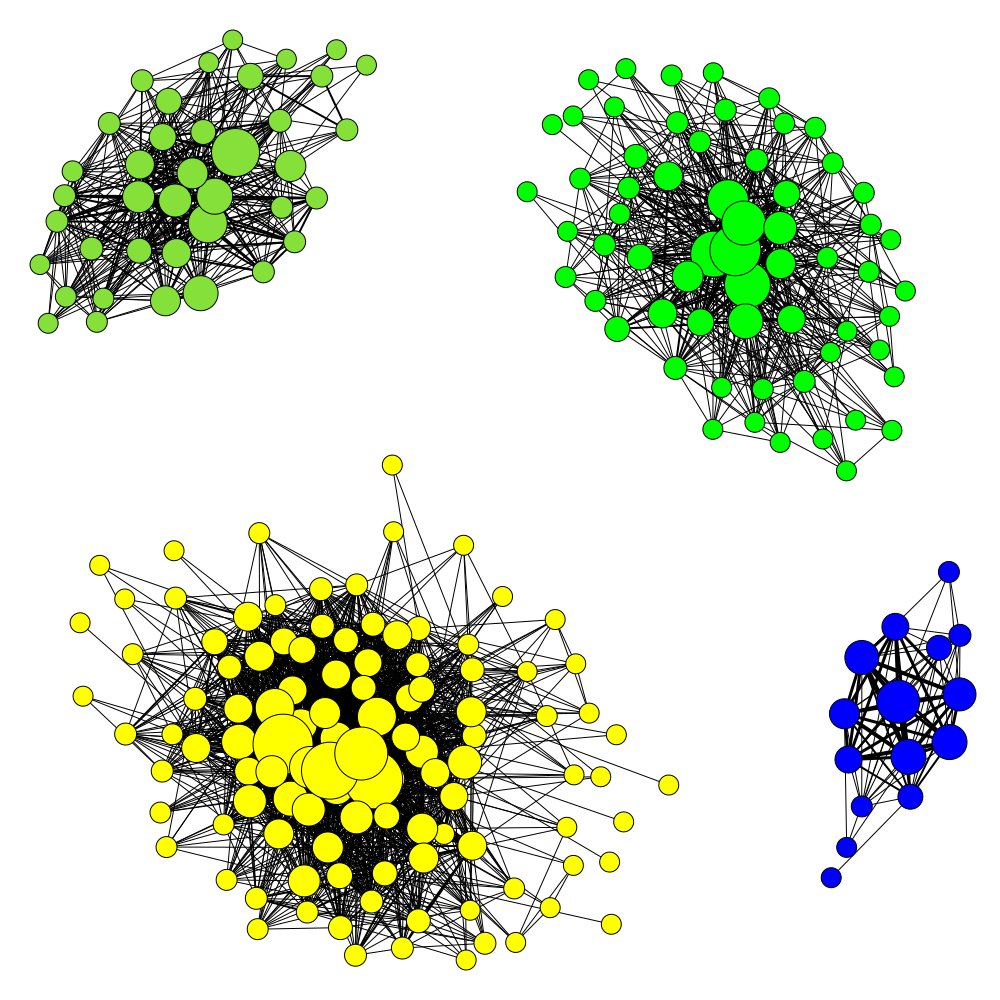
\includegraphics[width=12.5cm]{communities/topic_b_cs}}
    \caption[Visualisation of the community structure within the Topic network (Researchers as edges).]{Visualisation of the community structure within the Topic network (Researchers as edges).}
    \label{fig:topic_b_current_cs}
\end{figure}

\begin{table}[!htbp]
\centering
\caption[Number of nodes and the predominant words of each community identified in the Topic network (Researchers as edges) constructed using the current data set (2010 to 2016).]{Number of nodes and the predominant words based on word frequency of each community identified within the Topic network (Researchers as edges) constructed using the current data set (2010 to 2016).}
\label{table:topic_b_current_numbers}
\begin{tabular}{r|>{\raggedleft\arraybackslash}p{1.6cm}>{\raggedleft\arraybackslash}p{6.5cm}}
{} & \textbf{Number (topics)} & \textbf{Predominant words based on frequency of words}\\
\hline\\
\textbf{C1}  & {39}  & {engineering, management}\\
\textbf{C2}  & {62}  & {psychology, design}\\
\textbf{C3}  & {15}  & {mathematical, analysis}\\
\textbf{C4}  & {109} & {engineering, chemistry}\\
\hline\\
\textbf{All} & {225} & {engineering, management, science}\\
\end{tabular}
\end{table}

\subsection{Comparison of Grants and Researchers as edges}

There are obvious differences between the clustering produced using the \textit{Topic network (Grants as edges)} and \textit{Topic network (Researchers as edges)}. Firstly, the number of communities identified differs, as using the former 6 communities were identified, compared to 4 when using the latter. This results in an imbalance in community size, with one of the communities identified in the \textit{Topic network (Researcher as edges)} network consisting of 109 topics. A large community is also a broad community, which means that is less specific and lacks the capability to represent clear research areas. It also causes other communities to be significantly smaller in size.

Furthermore, using the \textit{Topic network (Researchers as edges)} network, the community with a evident focus in Mathematics is larger in size and its previous well-defined structure is "harmed" by the irrational addition of topics such as \textit{genomics}. Moreover, the clustering produced using the \textit{Researchers as edges interpretation} also failed in identifying the Biology-focused community, Community 1 in the \textit{Topic network (Grants as edges)}. However, there are also similarities between the community structures identified, as the \textit{engineering} and \textit{chemistry}-based communities appear in both.

In conclusion, this comparative analysis showed that the clustering produced using the \textit{Topic network (Grants as edges)} is more coherent and balanced than the one produced using the \textit{Topic network (Researchers as edges) network}.

\subsection{Evaluation of Topic clusters}

This section presents the results of the evaluation phase carried out on the identified topic clusters measuring the strength of the community structure identified in the \textit{Topic networks} (\textit{Grants as edges} and \textit{Researchers as edges}).

\subsubsection{Topic network (Grants as Edges)}

This section showcases the results of the evaluation phase. Pairs of nodes that are both from the same cluster and different clusters were identified. Moreover, the Average dice and Jaccard similarity between both types of node pairs was calculated. Table \ref{table:topic_a_evaluation} presents the results of the evaluation phase carried out on the Topic network (Grants as edges) constructed using both the historical (1990 to 2010) and current (2010 to 2016) data sets. The results show that nodes within the same cluster have a higher similarity than nodes from different clusters. This outcome also translates to the historical networks.

\begin{table}[htbp]
\centering
\caption[Dice and Jaccard similarity coefficients of node pairs within and between communities in the Topic network (Grants as edges) constructed using both the historical (1990 to 2010) and current (2010 to 2016) data sets.]{Dice and Jaccard similarity coefficients of node pairs within and between communities in the Topic network (Grants as edges) constructed using both the historical (1990 to 2010) and current (2010 to 2016) data sets. Each node pair represents an edge which connects two nodes within the same community or in two different communities. If the network division is strong, it is expected that a node pair within the same community will have a higher similarity compared to a node pair consisting of nodes from two different communities. \textit{IN} stands for within communities, while \textit{OUT} means between communities.}
\label{table:topic_a_evaluation}
\begin{tabular}{r|rrr}
{} & \textbf{1990-2000} & \textbf{2000-2010} & \textbf{2010-2016}\\
\hline\\
Node pairs IN                  & {437}   & {1940}  & {1122}\\
Node pairs OUT                 & {311}   & {1652}  & {886}\\
Average Dice similarity IN     & {0.465} & {0.510} & {0.428}\\
Average Dice similarity OUT    & {0.346} & {0.433} & {0.354}\\
Difference between IN and OUT  & {0.119} & {0.077} & {0.074}\\
Average Jaccard similarity IN  & {0.316} & {0.356} & {0.286}\\
Average Jaccard similarity OUT & {0.217} & {0.283} & {0.220}\\
Difference between IN and OUT  & {0.099} & {0.073} & {0.066}\\
\end{tabular}
\end{table}

\subsubsection{Topic network (Researchers as Edges)}

This section showcases the results of the evaluation phase. Pairs of nodes that are both from the same cluster and different clusters were identified. Moreover, the Average dice and Jaccard similarity between both types of node pairs was calculated. Table \ref{table:topic_b_evaluation} presents the results of the evaluation phase carried out on the Topic network (Researchers as edges) constructed using the current data set (2010 to 2016). The results show that nodes within the same cluster have a higher similarity than nodes from different clusters. This outcome also translates to the historical networks.

\begin{table}[htpb]
\centering
\caption[Dice and Jaccard similarity coefficients of node pairs within and between communities in the Topic network (Researchers as edges) constructed using the current data set (2010 to 2016).]{Dice and Jaccard similarity coefficients of node pairs within and between communities in the Topic network (Grants as edges) constructed using the current data set (2010 to 2016). Each node pair represents an edge which connects two nodes within the same community or in two different communities. If the network division is strong, it is expected that a node pair within the same community will have a higher similarity compared to a node pair consisting of nodes from two different communities. \textit{IN} stands for within communities, while \textit{OUT} means between communities.}
\label{table:topic_b_evaluation}
\begin{tabular}{r|r}
{} & \textbf{2010-2016}\\
\hline\\
Node pairs IN                  & {2921}\\
Node pairs OUT                 & {2271}\\
Average Dice similarity IN     & {0.543}\\
Average Dice similarity OUT    & {0.517}\\
Difference between IN and OUT  & {0.026}\\
Average Jaccard similarity IN  & {0.393}\\
Average Jaccard similarity OUT & {0.359}\\
Difference between IN and OUT  & {0.034}\\
\end{tabular}
\end{table}

\section{Networks of Researchers}

The other type of network created is a Network of Researchers. It consists of nodes which represent researchers and edges which are interpreted in two different ways, as they can either represent grants or topics. A separate network was constructed to fit each interpretation. They are referred to as \textit{Grants as edges} and \textit{Researchers as edges}. Moreover, as historical grant data was also collected, a further two versions of the Researcher network (Grants as edges) were constructed: 1990 to 2000 and 2000 to 2010, which resulted in a total of four constructed networks.

\subsection{Researcher network (Grants as edges)}

The \textit{Researcher network (Grants as edges)} is a carbon copy of the \textit{Topic network (Grants as edges)}, with the exception that nodes represent researchers and not topics. Its current data-based form is composed of 260 nodes and 208 edges representing one or more common grants between two researchers. Fig. \ref{fig:researcher_b_vis} showcases the visualisation of this network, indicating the network's heavily disconnected structure primarily due to the rarity in repeated collaboration between researchers on EPSRC-supported research grants which may last up to 8 years.

\begin{figure}[htpb]
    \centering
    \fbox{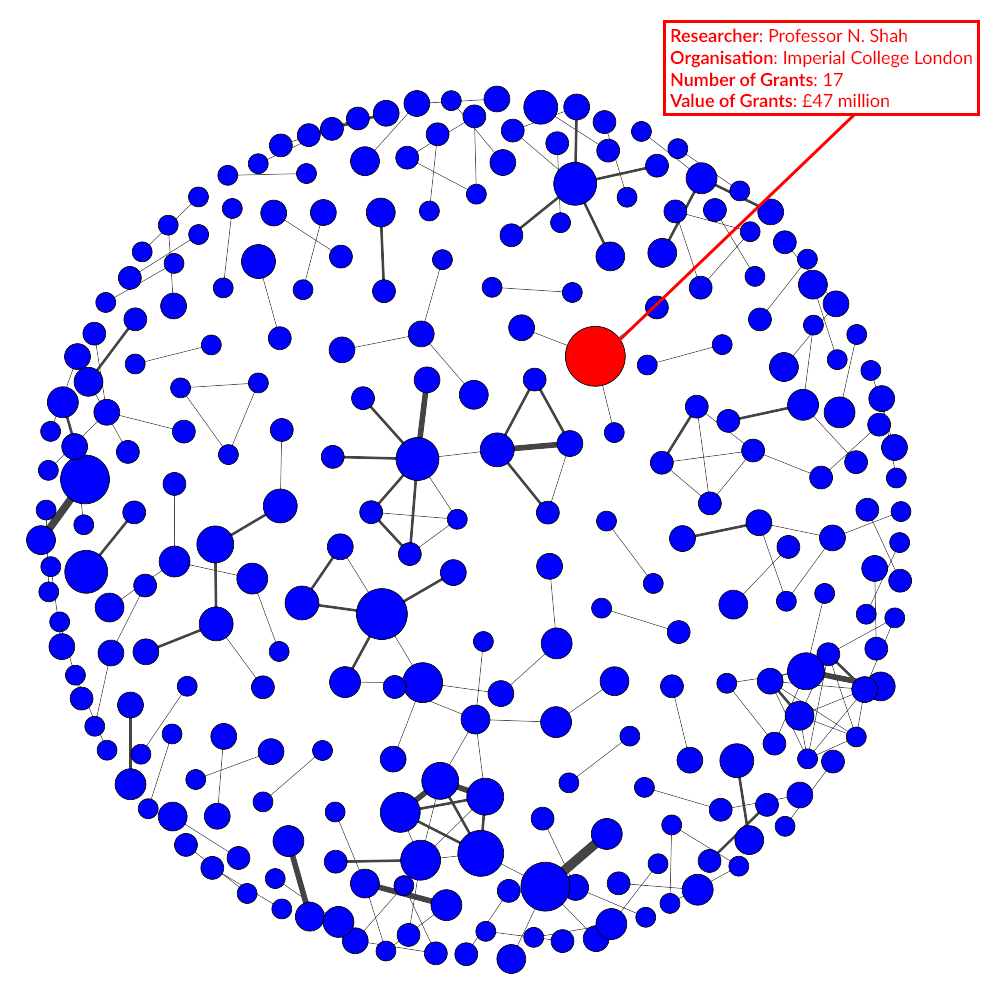
\includegraphics[width=12.5cm]{networks/researcher_b}}
    \caption{Visualisation of Researcher network (Grants as edges) constructed using the current data set (2010 to 2016). Node coloured in red represents the researcher involved in most grants.}
    \label{fig:researcher_b_vis}
\end{figure}

Furthermore, its historical data-based form consists of both an increased number of nodes and edges. The network is weighted, with its edge weight attribute representing the number of grants that two researchers have in common. Table \ref{table:researcher_b_stats} presents the statistics of the Researcher networks (Grants as edges).

\begin{table}[htbp]
\centering
\caption[Statistics of the Researcher network (Grants as edges) constructed using both the historical (1990 to 2010) and current (2010 to 2016) data sets]{Statistics of the Researcher network (Grants as edges) constructed using both the current and historical data sets (1990 to 2010).}
\label{table:researcher_b_stats}
\begin{tabular}{r|rrr}
{} & \textbf{1990-2000} & \textbf{2000-2010} & \textbf{2010-2016}\\
\hline\\
\textbf{Nodes}                          & {1847}   & {2434}    & {260}\\
\textbf{Edges}                          & {2002}   & {4919}    & {208}\\
\textbf{Type}                           & {Undirected} & {Undirected} & {Undirected}\\
\textbf{Weighted}                       & {Yes}    & {Yes}     & {Yes}\\
%\textbf{Connected}                     & {No}     & {No}      & {No}\\
\textbf{Average Degree}                 & {2.168}  & {4.042}   & {1.60}\\
\textbf{Average Weighted Degree}        & {2.798}  & {7.794}   & {2.592}\\
\textbf{Diameter}                       & {18.0}   & {36.0}    & {16.0}\\
%\textbf{Radius}                        & {1.0}    & {1.0}     & {1.0}\\
\textbf{Density}                        & {0.001}  & {0.002}   & {0.006}\\
\textbf{Modularity}                     & {0.978}  & {0.977}   & {0.955}\\
%\textbf{Communities}                   & {563}    & {485}     & {91}\\
\textbf{Weak Components}                & {559}    & {473}     & {89}\\
%\textbf{Node Closeness}                & {0.001}  & {0.0}     & {0.004}\\
%\textbf{Node Betweenness}              & {14.214} & {138.711} & {1.965}\\
%\textbf{Edge Betweenness}              & {17.545} & {79.157}  & {4.625}\\
\textbf{Average Clustering Coefficient} & {0.648}  & {0.748}   & {0.578}\\
%\textbf{Eigenvector Centrality}        & {0.005}  & {0.007}   & {0.016}\\
\textbf{Average Path Length}            & {3.676}  & {6.874}   & {1.942}\\
\end{tabular}
\end{table}

\subsection{Researcher network (Topics as edges)}

The \textit{Researcher network (Topics as edges)} is a reversed version of the \textit{Topic network (Researchers as edges)}. It consists of 655 researchers linked by 4548 edges representing common topics between the researchers. The network is undirected and weighted with the edge weight representing the number of topics two researchers have in common. In comparison to current version of the \textit{Researcher network (Grants as edges)} which consists of 260 nodes and 208 edges, this network consists of substantially more nodes and edges. Table \ref{table:researcher_a_stats} presents the statistics of the Researcher network (Topics as edges).

\begin{table}[htbp]
\centering
\caption{Statistics of the Researcher network (Topics as edges).}
\label{table:researcher_a_stats}
\begin{tabular}{r|r}
{} & \textbf{2010-2016}\\
\hline\\
\textbf{Nodes}                          & {655}\\
\textbf{Edges}                          & {4548}\\
\textbf{Type}                           & {Undirected}\\
\textbf{Weighted}                       & {Yes}\\
%\textbf{Connected}                     & {No}\\
\textbf{Average Degree}                 & {13.887}\\
\textbf{Average Weighted Degree}        & {27.258}\\
\textbf{Diameter}                       & {15.0}\\
%\textbf{Radius}                        & {1.0}\\
\textbf{Density}                        & {0.021}\\
\textbf{Modularity}                     & {0.738}\\
%\textbf{Communities}                   & {49}\\
\textbf{Weak Components}                & {39}\\
%\textbf{Node Closeness}                & {0.005}\\
%\textbf{Node Betweenness}              & {703.138}\\
%\textbf{Edge Betweenness}              & {127.386}\\
\textbf{Average Clustering Coefficient} & {0.825}\\
%\textbf{Eigenvector Centrality}        & {0.078}\\
\textbf{Average Path Length}            & {4.278}\\
\end{tabular}
\end{table}

\begin{figure}[htpb]
    \centering
    \fbox{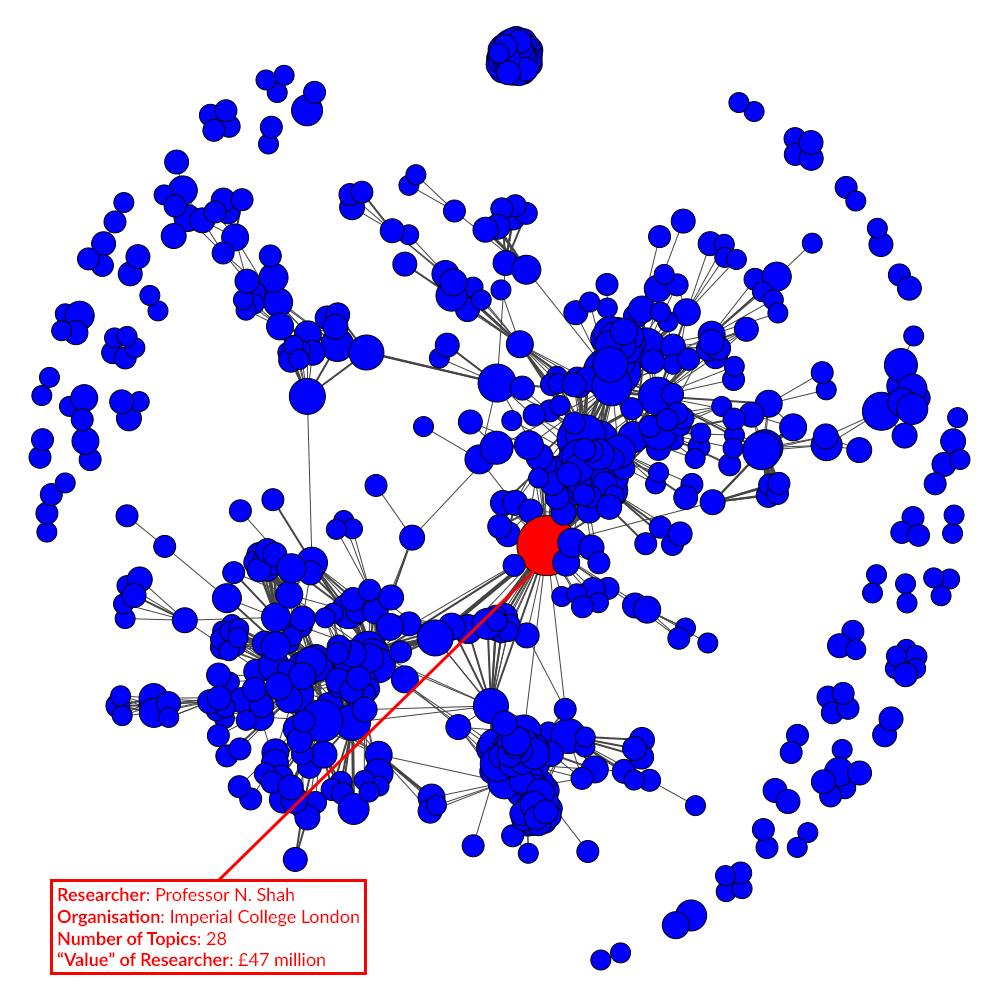
\includegraphics[width=12.5cm]{networks/researcher_a}}
    \caption{Visualisation of the Researcher network (Grants as edges). Node coloured in red represents the researcher that has the most topics.}
    \label{fig:researcher_a_vis}
\end{figure}

As illustrated in Fig. \ref{fig:researcher_a_vis}, the structure of this network stands out from the others. In one hand, both Topic networks feature a conglomeration of nodes densely connected. On the other hand, the Researcher network (Grants as edges) consists the opposite of that, sparsely connected with up to maximum of 4 connected nodes. The structure of the \textit{Researcher network (Topics as edges)} is a combination between the two. Based on an initial observation, a not so surprising guess would indicate that a community detection algorithm has already been applied to this network. However it hasn't, as its structure clearly showcases the layout of collaboration between EPSRC-supported researchers. Several relatively small groups of researchers, densely connected to one another, but otherwise sparsely connected, can be spotted. Another guess would be the assumption that the communities represent common topic interests between researchers.

\section{Clusters of Researchers}

The previous two sections presented part of the second batch of results that the project produced which is the \textit{Networks of Researchers}. The optimal solution identified at the end of the comparison experiments stage was applied to the networks constructed, which resulted in a number researcher clusters. This section presents and discusses the results produced using both \textit{Researcher networks}, \textit{Grants} and \textit{Topics as edges}.

\subsection{Researcher network (Grants as edges)}

The application of the Louvain community detection algorithm on the \textit{Researcher network (Grants as edges)} resulted in the initial and excessive identification of 89 communities of researchers. This is due to the lack of strong and frequent relationships between researchers. Note that the \textit{Researcher network (Grants as edges)} consists of researchers linked by their common grants. Also note that, during the network creation process, due to the magnitude of the network, the \textit{Researcher network (Grants as edges)} was sampled and only includes researchers that have two or more grants in common. This threshold represents a fairly strong collaboration link between two researchers.

In conclusion, it seems that two or more researchers collaborating multiple times as part of a grant is a rarity within the EPSRC data. Due to the sparse nature of the communities identified, only the two largest communities are presented here. Fig. \ref{fig:researcher_b_current_cs} showcases the visualisation of the identified community structure within this network. Table \ref{table:researcher_b_current_numbers} presents the number of nodes representing researchers and the number and value of grants within each community in the \textit{Researcher network (Grants as edges)} constructed using the current data set (2010 to 2016). The complete clustering of the Researcher network (Grants as edges) constructed using the current data set (2010 to 2016) is presented in Table \ref{table:researcher_b_current_clusters_appendix} which is part of Appendix \ref{appendix:data}.

\begin{figure}[htpb]
    \centering
    \fbox{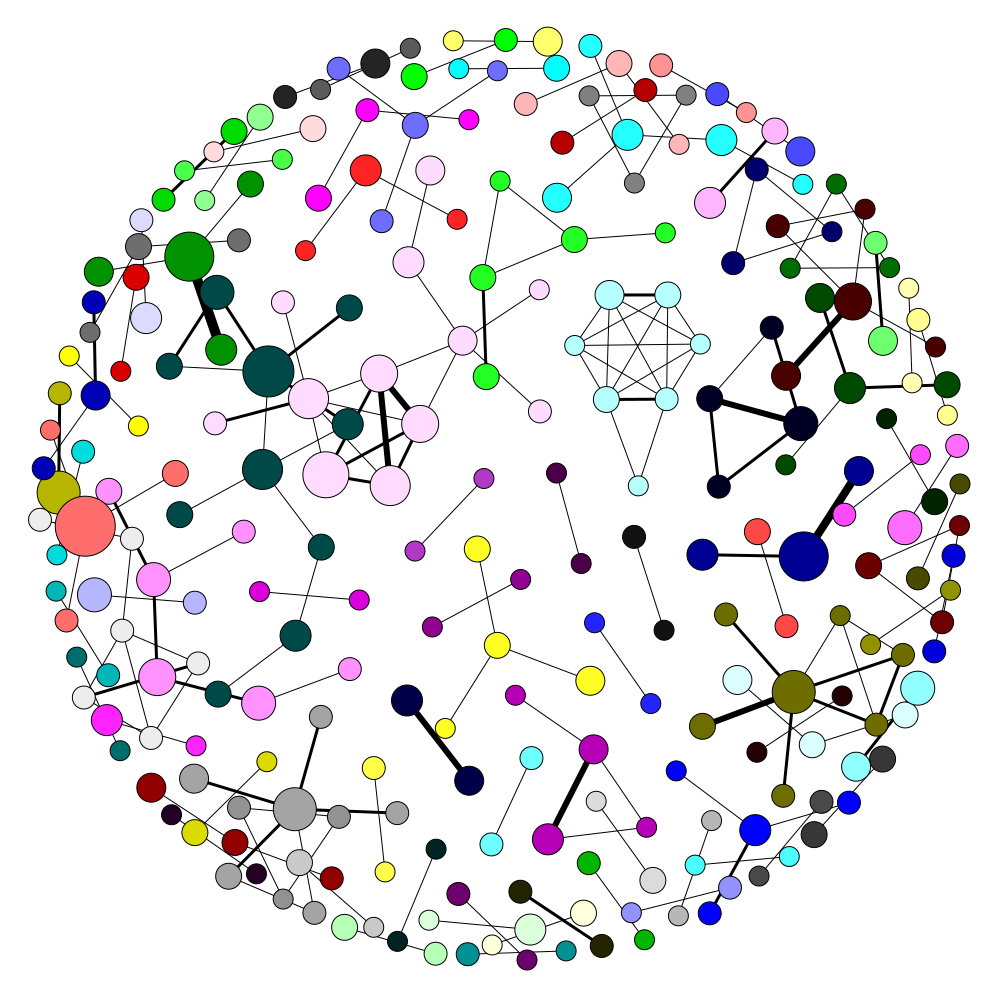
\includegraphics[width=12.5cm]{communities/researcher_b_cs}}
    \caption[Visualisation of the community structure within the Researcher network (Grants as edges) constructed using the current data set (2010 to 2016).]{Visualisation of the community structure within the Researcher network (Grants as edges) constructed using the current data set (2010 to 2016).}
    \label{fig:researcher_b_current_cs}
\end{figure}

\begin{table}[!htbp]
\centering
\caption[Number of nodes and grants and value of grants in each community within the Researcher network (Grants as edges) constructed using the current data set (2010 to 2016).]{Number of nodes and grants and value of grants in each community identified within the Researcher network (Grants on edges) constructed using the current data set (2010 to 2016). The number of grants includes duplicate grants, as a grant can be part of more than one community. Subsequently, the value of grants also includes the duplicate grants. However, the last column represents the number and value of unique grants in communities within the current Researcher network (Grants on edges).}
\label{table:researcher_b_current_numbers}
\begin{tabular}{r|rrrr}
{} & \textbf{C1} & \textbf{C2} & \textbf{Total}\\
\hline\\
\textbf{Number of researchers} & {10} & {12} & {22}\\
\textbf{Number of grants}      & {33} & {35} & {65}\\
\textbf{Value of grants} & {\pounds103M} & {\pounds87M} & {\pounds177M}\\
\end{tabular}
\end{table}

\subsubsection{Historical data comparison}

Similar to the historical data comparison of the Topic network, there is a clear funding trend which increases more rapidly the more recent the grant is. Currently, there are 65 grants within the two largest communities worth a total value of \pounds3.5B. Table \ref{table:researcher_b_past1_numbers} presents the number of nodes representing researchers and the number and value of grants within each community in the \textit{Researcher network (Grants as edges)} constructed using the historical data set (2000 to 2010).

\begin{table}[!htbp]
\centering
\caption[Number of nodes and grants and value of grants in each community within the Researcher network (Grants as edges) constructed using the current data set (2000 to 2010).]{Number of nodes and grants and value of grants in each community identified within the Researcher network (Grants on edges) constructed using the current data set (2000 to 2010). The number of grants includes duplicate grants, as a grant can be part of more than one community. Subsequently, the value of grants also includes the duplicate grants. However, the last column represents the number and value of unique grants in communities within the current Researcher network (Grants on edges).}
\label{table:researcher_b_past1_numbers}
\begin{tabular}{r|rrrrr}
{} & \textbf{C1} & \textbf{C2} & \textbf{C3} & \textbf{C4} & \textbf{Total}\\
\hline\\
\textbf{Number of researchers} & {49}  & {46}  & {55}  & {65}  & {215}\\
\textbf{Number of grants}      & {213} & {184} & {208} & {278} & {866}\\
\textbf{Value (grants)} & {\pounds87M} & {\pounds123M} & {\pounds136M} & {\pounds234M} & {\pounds551M}\\
\end{tabular}
\end{table}

Between, 2010-2000, researchers worked on 866 grants, valued at \pounds551M. These figures indicate a significant difference in the number of grants. However, this is justified, as the two time periods compared are not equal, as the former covers 6 years of grants, while the latter covers 10 years. More importantly, the difference in value is not considerable, which shows the progress of research funding over the years, as current grants received significantly more funding. Furthermore, this is supported by the number and value of the grants from 1990 to 2000.  Researchers worked on a slightly less number of grants than between 2000 and 2010, but they also received significantly less funding, \pounds130M. Table \ref{table:researcher_b_past2_numbers} presents the number of nodes representing researchers and the number and value of grants within each community in the \textit{Researcher network (Grants as edges)} constructed using the historical data set (1990 to 2000).

\begin{table}[!htbp]
\centering
\caption[Number of nodes and grants and value of grants in each community within the Researcher network (Grants as edges) constructed using the current data set (1990 to 2000).]{Number of nodes and grants and value of grants in each community identified within the Researcher network (Grants on edges) constructed using the current data set (1990 to 2000). The number of grants includes duplicate grants, as a grant can be part of more than one community. Subsequently, the value of grants also includes the duplicate grants. However, the last column represents the number and value of unique grants in communities within the current Researcher network (Grants on edges).}
\label{table:researcher_b_past2_numbers}
\begin{tabular}{r|rrrrrr}
{} & \textbf{C1} & \textbf{C2} & \textbf{C3} & \textbf{C4} & \textbf{C5} & \textbf{Total}\\
\hline\\
\textbf{Number of researchers} & {31}  & {21} & {46}  & {35}  & {30}  & {163}\\
\textbf{Number of grants}      & {115} & {78} & {150} & {147} & {129} & {610}\\
\textbf{Value of grants} & {\pounds34M} & {\pounds18M} & {\pounds21M} & {\pounds41M} & {\pounds17M} & {\pounds130M}
\end{tabular}
\end{table}

\subsection{Researcher network (Topics as edges)}

In contrast to the Researcher network (Grants as edges), the application of the Louvain community detection algorithm on the \textit{Researcher network (Topics as edges)} resulted in the less excessive initial identification of 49 communities of researchers. However, the number of identified communities is still too large and represents communities consisting of small numbers of researchers that have a small number of topics in common. Note that the \textit{Researcher network (Topics as edges)} consists of researchers linked by their common topics. Also note that, during the network creation process, due to the magnitude of the network, the \textit{Researcher network (Topics as edges)} was sampled and only includes researchers that have at least five topics in common. This threshold represents a strong topic interest linking two researchers.

In conclusion, it seems that a large number of researchers having multiple common topics is a rarity within the EPSRC data. Due to the sparse nature of the communities identified, the eight largest communities are presented here. Fig. \ref{fig:researcher_a_current_cs} showcases the visualisation of the identified community structure within this network. Table \ref{table:researcher_a_current_numbers} presents the number of nodes representing topics within each community in the \textit{Researcher network (Topics as edges)}). The complete clustering of the Researcher network (Topics as edges) constructed using the current data set (2010 to 2016) is presented in Table \ref{table:researcher_a_current_clusters_appendix} which is part of Appendix \ref{appendix:data}.

\begin{figure}[!htpb]
    \centering
    \fbox{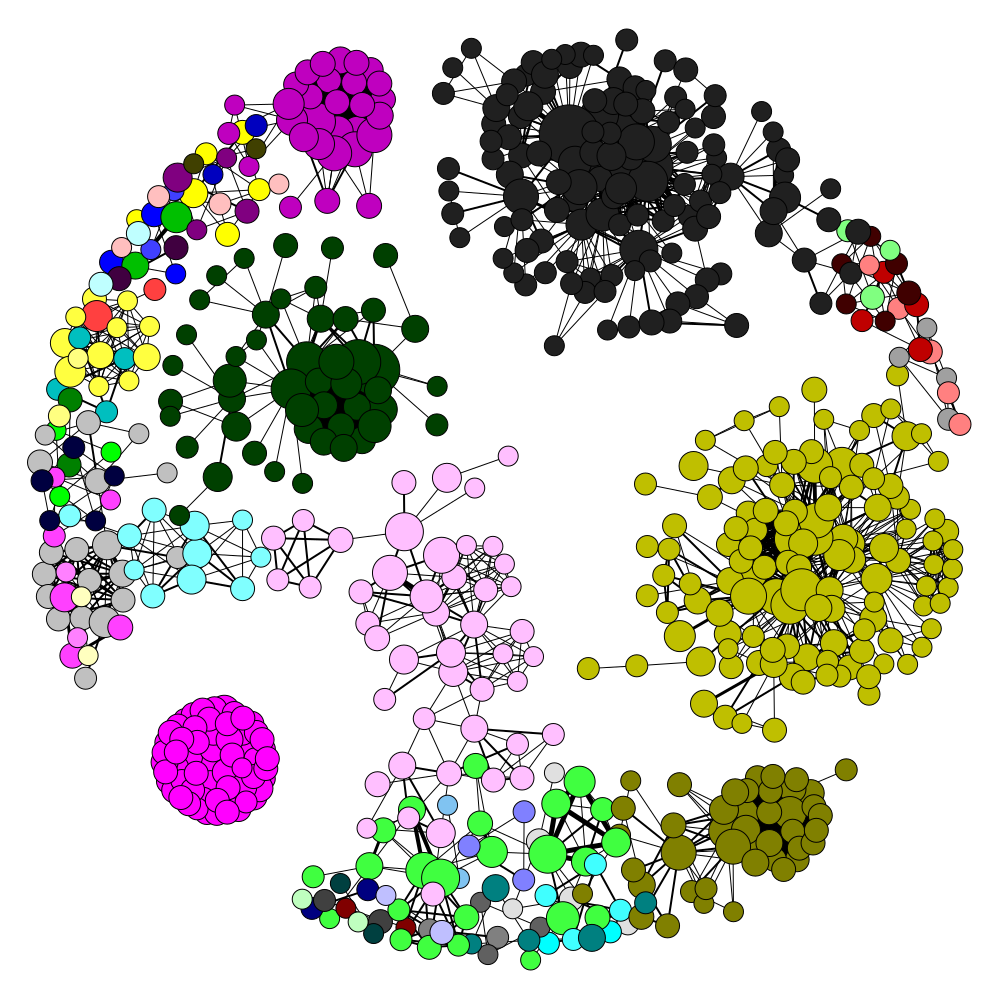
\includegraphics[width=12.5cm]{communities/researcher_a_cs}}
    \caption[Visualisation of the community structure within the Researcher network (Topics as edges).]{Visualisation of the community structure within the Topic network (Researchers as edges).}
    \label{fig:researcher_a_current_cs}
\end{figure}

\begin{table}[!htbp]
\centering
\caption[Number of nodes in each community within the Researcher network (Topics as edges) constructed using the current data set (2010 to 2016).]{Number of nodes in each community identified within the Researcher network (Grants on edges) constructed using the current data set (2010 to 2016).}
\label{table:researcher_a_current_numbers}
\begin{tabular}{r|rrrrrrrrr}
{} & \textbf{C1} & \textbf{C2} & \textbf{C3} & \textbf{C4} & \textbf{C5} & \textbf{C6} & \textbf{C7} & \textbf{C8} & \textbf{Total}\\
\hline\\
\textbf{Number of researchers} & {60} & {120} & {30} & {24} & {43} & {48} & {126} & {46} & {225}
\end{tabular}
\end{table}

\subsection{Comparison of Grants and Topics as edges}

The results produced using both networks clearly indicate that the \textit{Researcher network (Topics as edges)} is the more rational and successful interpretation of the data, as expected prior to creation process of the Researcher network.

In one hand, a network that consists of researchers and links between them symbolising a work collaboration between the two. As proved by the results, this is fairly rare in the academic world. Unless two researchers have a relationship, are part of the same institution or organisation or are located in the same city, it is hard to believe that they would collaborate on multiple occasions. Moreover, it is essential to note that there is a clear difference between collaborating on a government-funded grant and any other research project. Certain grants can last up to 7 years and at the end of the grant the researchers that worked on it will most probably not collaborative again for a lengthy period of time if at all. In conclusion, the grant-based interpretation of the researcher data did not prove to be significantly valuable. However it did provide interesting insights into the progress of funding over a 26-year long period.

On the other hand, a network that consists of researchers and links between them symbolising a shared research interest between the two. This type of connection between two researchers is not limited to sharing a relationship, institution or organisation or location. Only a shared research interest is required. In the academic world, this is very common as researchers from all over the world can related to each other through a common research field. The ideal result from such a network is a fairly low number of communities consisting of researchers that share an interest in a number of different topics. However, due to the large number of researchers, the number of identified communities is also large and at the same time sparse. That being said, this interpretation of the data is still better, as it produces a more coherent clustering based on the researcher data available.

\subsection{Evaluation of Researcher clusters}

This section presents the results of the evaluation phase carried out on the identified researcher clusters in order to measure the strength of the community structure identified in the \textit{Researcher networks} (\textit{Grants as edges} and \textit{Topics as edges}).

\subsubsection{Researcher network (Grants as Edges)}

This section showcases the results of the evaluation phase. Pairs of nodes that are both from the same cluster and different clusters were identified. Moreover, the Average dice and Jaccard similarity between both types of node pairs was calculated. Table \ref{table:researcher_b_evaluation} presents the results of the evaluation phase carried out on the Researcher network (Researchers as edges) constructed using both the historical (1990 to 2010) and current (2010 to 2016) data sets. The results show that nodes within the same cluster have a higher similarity than nodes from different clusters. This outcome also translates to the historical networks.

\begin{table}[htpb]
\centering
\caption[Dice and Jaccard similarity coefficients of node pairs within and between communities in the Researcher network (Grants as edges) constructed using both the historical (1990 to 2010) and current (2010 to 2016) data sets.]{Dice and Jaccard similarity coefficients of node pairs within and between communities in the Researcher network (Grants as edges) constructed using both the historical (1990 to 2010) and current (2010 to 2016) data sets. Each node pair represents an edge which connects two nodes within the same community or in two different communities. If the network division is strong, it is expected that a node pair within the same community will have a higher similarity compared to a node pair consisting of nodes from two different communities. \textbf{IN} stands for within communities, while \textbf{OUT} means between communities.}
\label{table:researcher_b_evaluation}
\begin{tabular}{r|rrr}
{} & \textbf{1990-2000} & \textbf{2000-2010} & \textbf{2010-2016}\\
\hline\\
Node pairs IN                  & {1992}  & {4901}  & {206}\\
Node pairs OUT                 & {10}    & {18}    & {2}\\
Average Dice similarity IN     & {0.840} & {0.825} & {0.823}\\
Average Dice similarity OUT    & {0.342} & {0.321} & {0.336}\\
Difference between IN and OUT  & {0.481} & {0.504} & {0.505}\\
Average Jaccard similarity IN  & {0.736} & {0.740} & {0.762}\\
Average Jaccard similarity OUT & {0.210} & {0.200} & {0.202}\\
Difference between IN and OUT  & {0.526} & {0.540} & {0.560}\\
\end{tabular}
\end{table}

\subsubsection{Researcher network (Topics as Edges)}

This section showcases the results of the evaluation phase. Pairs of nodes that are both from the same cluster and different clusters were identified. Moreover, the Average dice and Jaccard similarity between both types of node pairs was calculated. Table \ref{table:researcher_a_evaluation} presents the results of the evaluation phase carried out on the Researcher network (Topics as edges) constructed using the current data set (2010 to 2016). The results show that nodes within the same cluster have a higher similarity than nodes from different clusters. This outcome also translates to the historical networks.

\begin{table}[htpb]
\centering
\caption[Dice and Jaccard similarity coefficients of node pairs within and between communities in the Researcher network (Topics as edges) constructed using the current data set (2010 to 2016).]{Dice and Jaccard similarity coefficients of node pairs within and between communities in the Researcher network (Topics as edges) constructed using the current data set (2010 to 2016). Each node pair represents an edge which connects two nodes within the same community or in two different communities. If the network division is strong, it is expected that a node pair within the same community will have a higher similarity compared to a node pair consisting of nodes from two different communities. \textit{IN} stands for within communities, while \textit{OUT} means between communities.}
\label{table:researcher_a_evaluation}
\begin{tabular}{r|r}
{} & \textbf{2010-2016}\\
\hline\\
Node pairs IN                  & {4273}\\
Node pairs OUT                 & {275}\\
Average Dice similarity IN     & {0.835}\\
Average Dice similarity OUT    & {0.405}\\
Difference between IN and OUT  & {0.430}\\
Average Jaccard similarity IN  & {0.779}\\
Average Jaccard similarity OUT & {0.273}\\
Difference between IN and OUT  & {0.506}\\
\end{tabular}
\end{table}